\chapter{Fringe field compensation using solenoids} \label{app-C}

In this appendix, we illuminate the finding from \cite{Holmes2018} that in an otherwise linear lattice with equal tunes, nonlinear fringe fields tend to eliminate any cross-plane correlations in the beam, but that this effect can be mitigated by solenoid magnetic fields and/or the beam's electric field.

To demonstrate this, a Danilov distribution matched to a linearized version of the SNS ring was generated. Fringe fields were turned on and the distribution was tracked without space charge. Fig.~\ref{fig:fringe_a} shows the turn-by-turn evolution.

There is nonlinear coupling between the horizontal and vertical motion, and the final distribution is a superposition of rotating and counter-rotating modes. We take this to be due to the difference resonance $\nu_x - \nu_y \approx 0$. In Fig.~\ref{fig:fringe_b}, a solenoid magnet is added to the ring. The cross-plane correlations are now mostly maintained. One explanation for this phenomenon is that since the solenoid is a coupled element, it splits the tunes of the system — $\nu_{x, y} \rightarrow \nu_{1, 2}$ with $\nu_1 \ne \nu_2$ — so the difference resonance is avoided.

In Fig.~\ref{fig:fringe_c}, the simulation is repeated with the inclusion of space charge instead of the solenoid magnet. An intensity of $10^{14}$ is used and the bunch length is equal to the ring length. Since the beam's electric field also introduces linear coupled forces, space charge has a stabilizing effect like that of the solenoid magnetic field.

It is recommended, however, that solenoid magnets be added to the SNS ring to produce a Danilov-like distribution using the elliptical painting method. The difficulty is that fringe fields seem to dominate at the beginning of injection when the transverse displacement is maximum and before a round beam has been formed. Additionally, without a solenoid in the ring, the quality of the final distribution is very sensitive to the difference in horizontal and vertical tunes. With a solenoid in the ring, elliptical trajectories at the injection point are produced for a wide range of original horizontal and vertical tunes. 


\begin{figure}[!p]
    \centering
    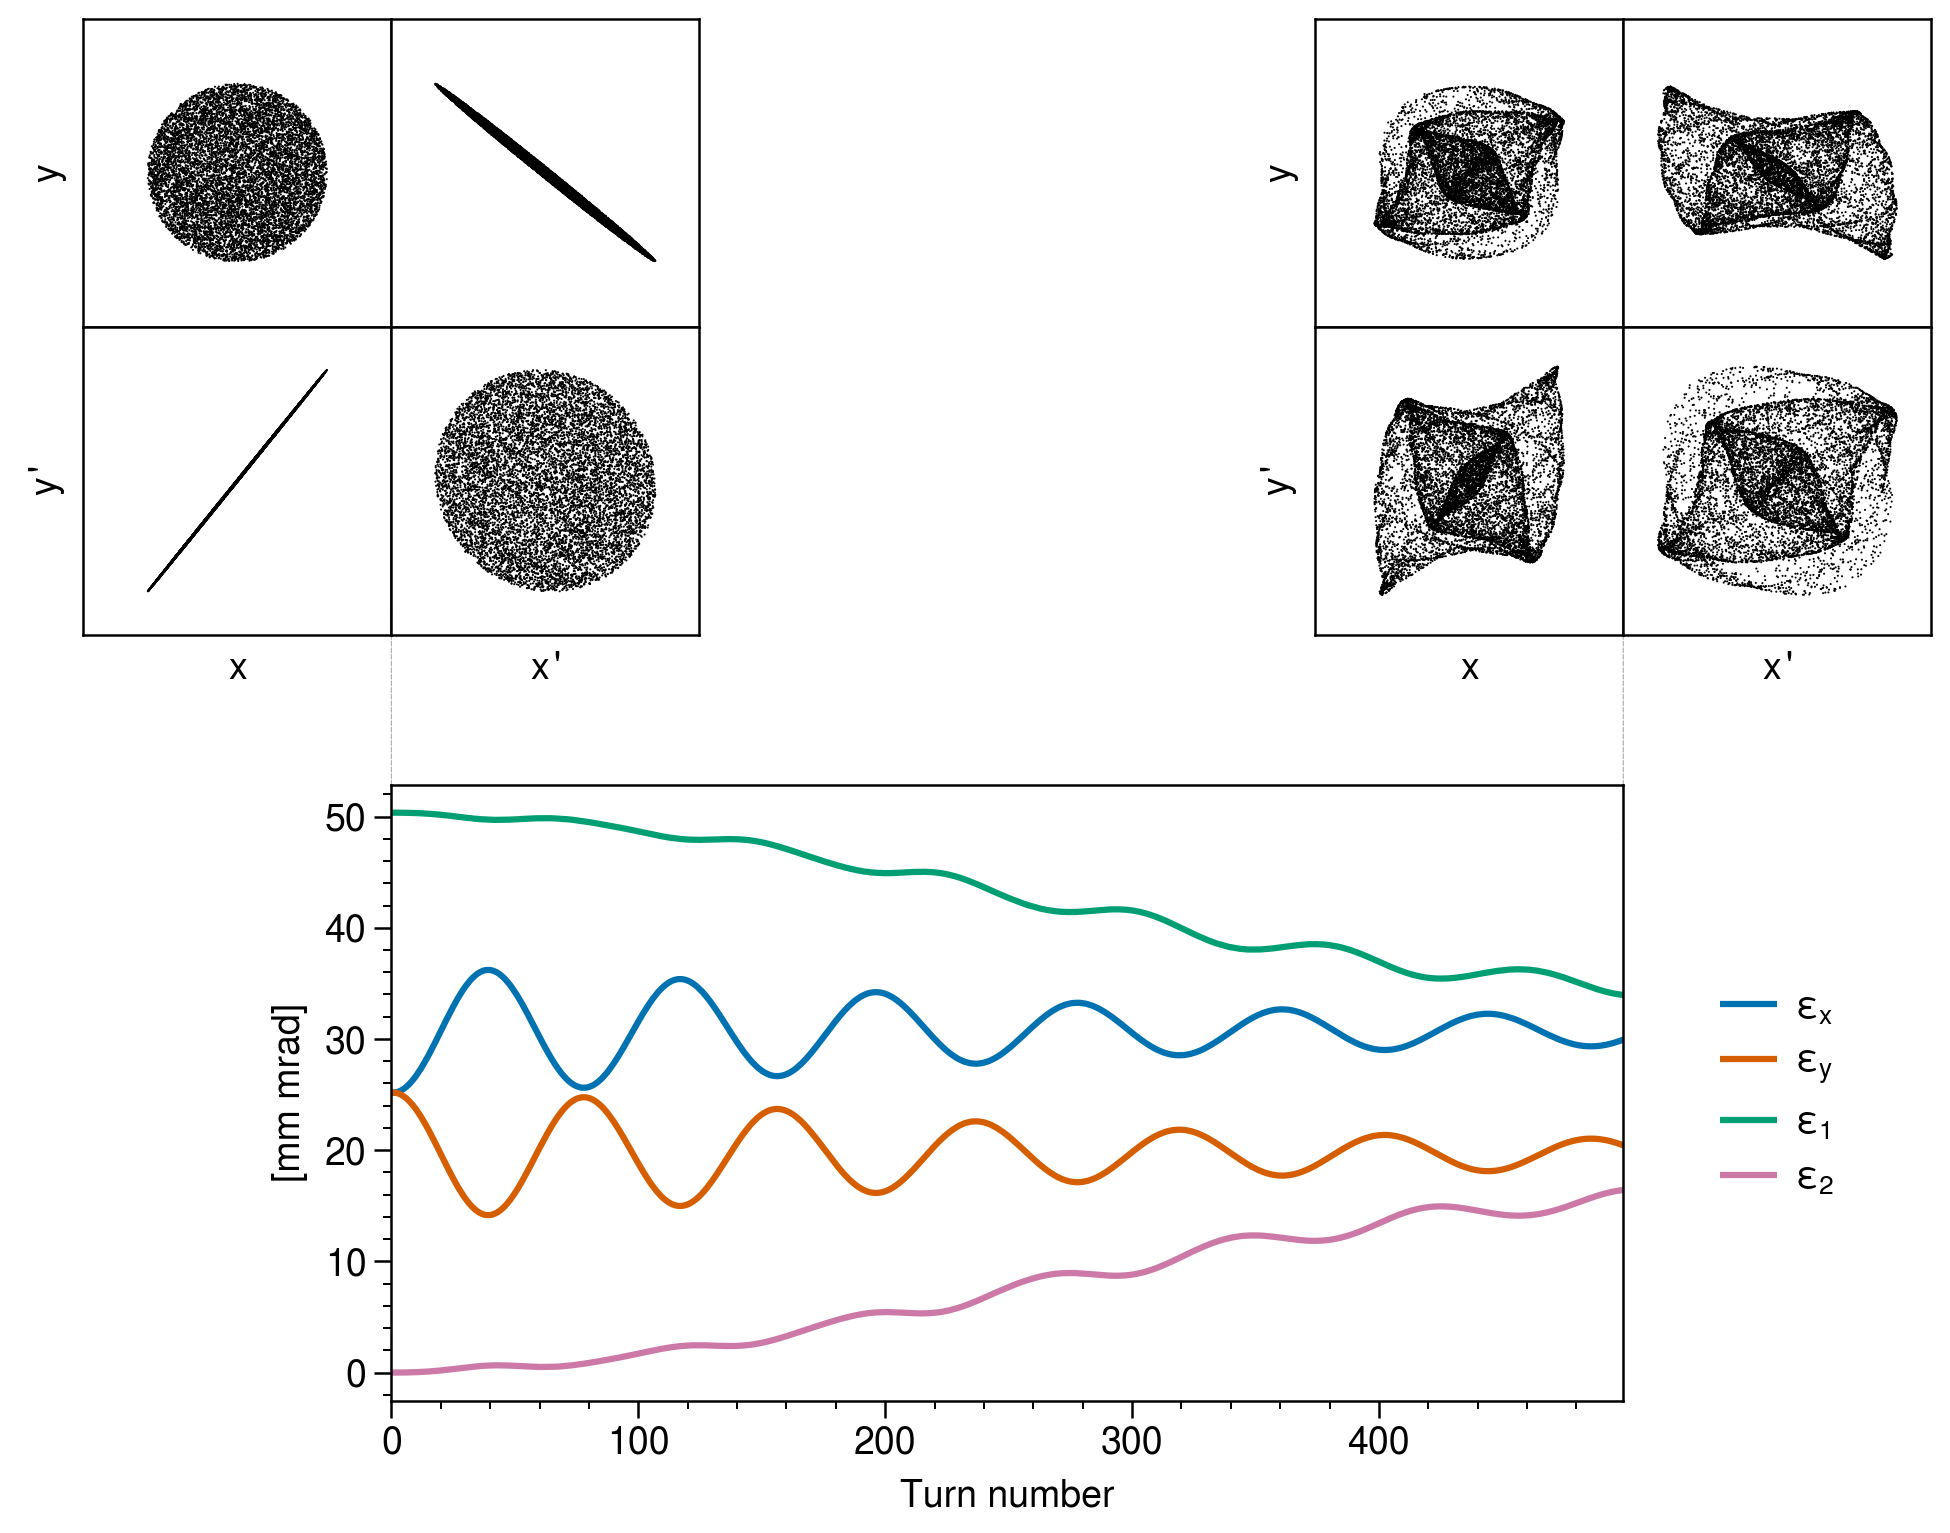
\includegraphics[width=0.7\textwidth]{Images/chapter3/fringe.png}
    \caption{Danilov distribution tracked in the SNS ring. Fringe fields are the only nonlinear external effect.}
    \label{fig:fringe_a}
    \vspace*{3cm}
\end{figure}

\begin{figure}[!p]
    \centering
    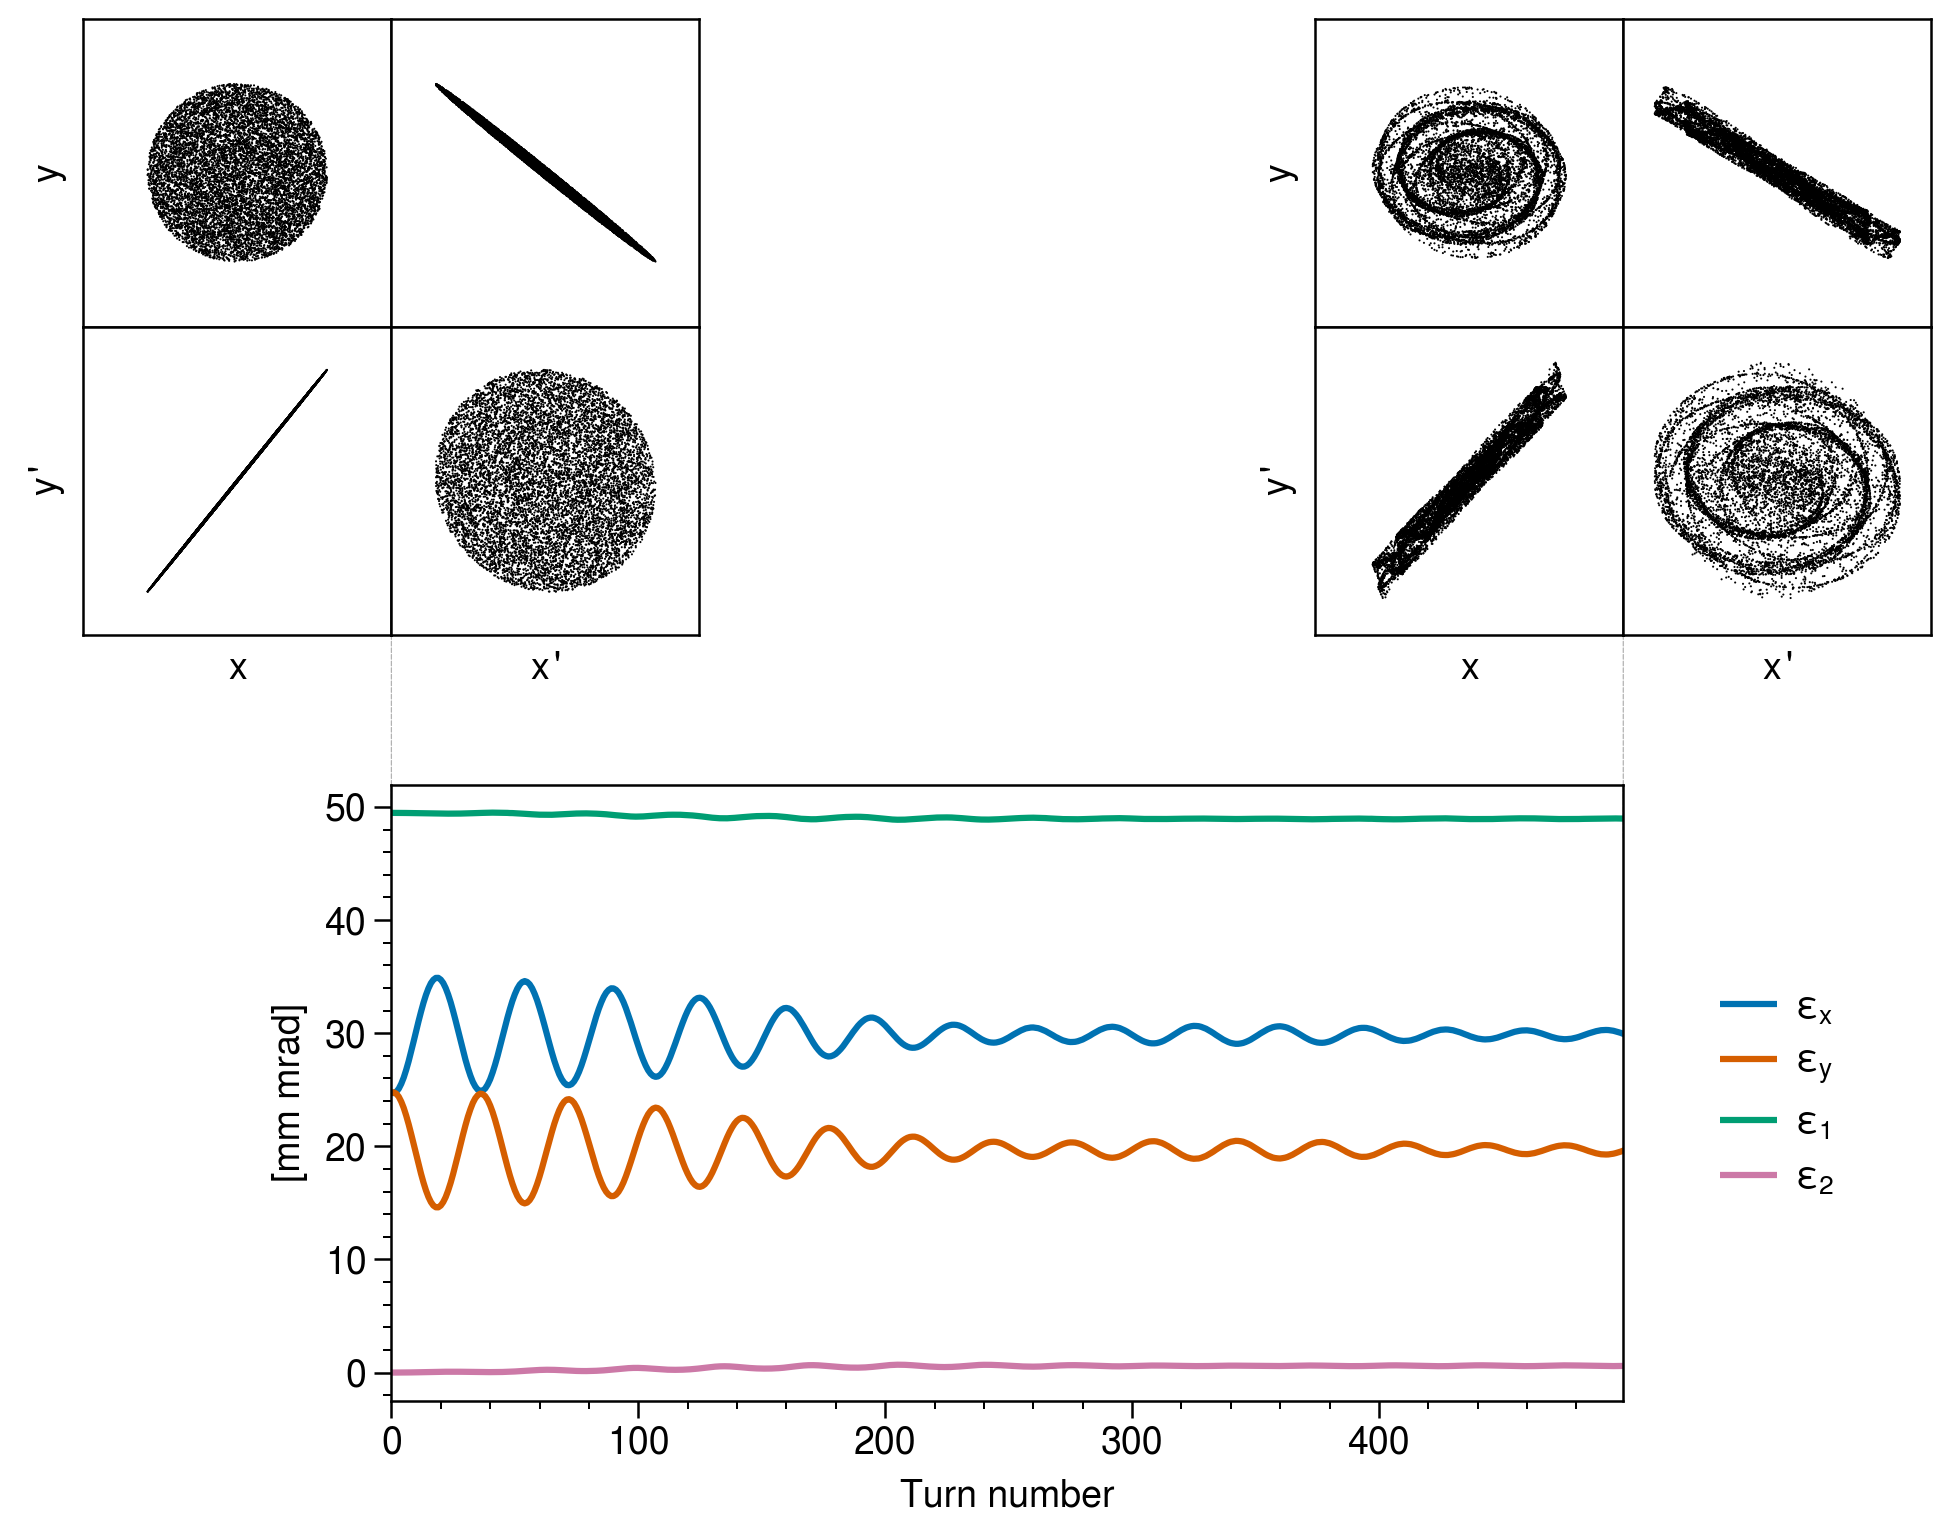
\includegraphics[width=0.7\textwidth]{Images/chapter3/fringe_solenoid.png}
    \caption{Danilov distribution tracked in the SNS ring with a solenoid added to the ring. Fringe fields are the only nonlinear external effect.}
    \label{fig:fringe_b}
    \vspace*{3cm}
\end{figure}

\begin{figure}[!p]
    \centering
    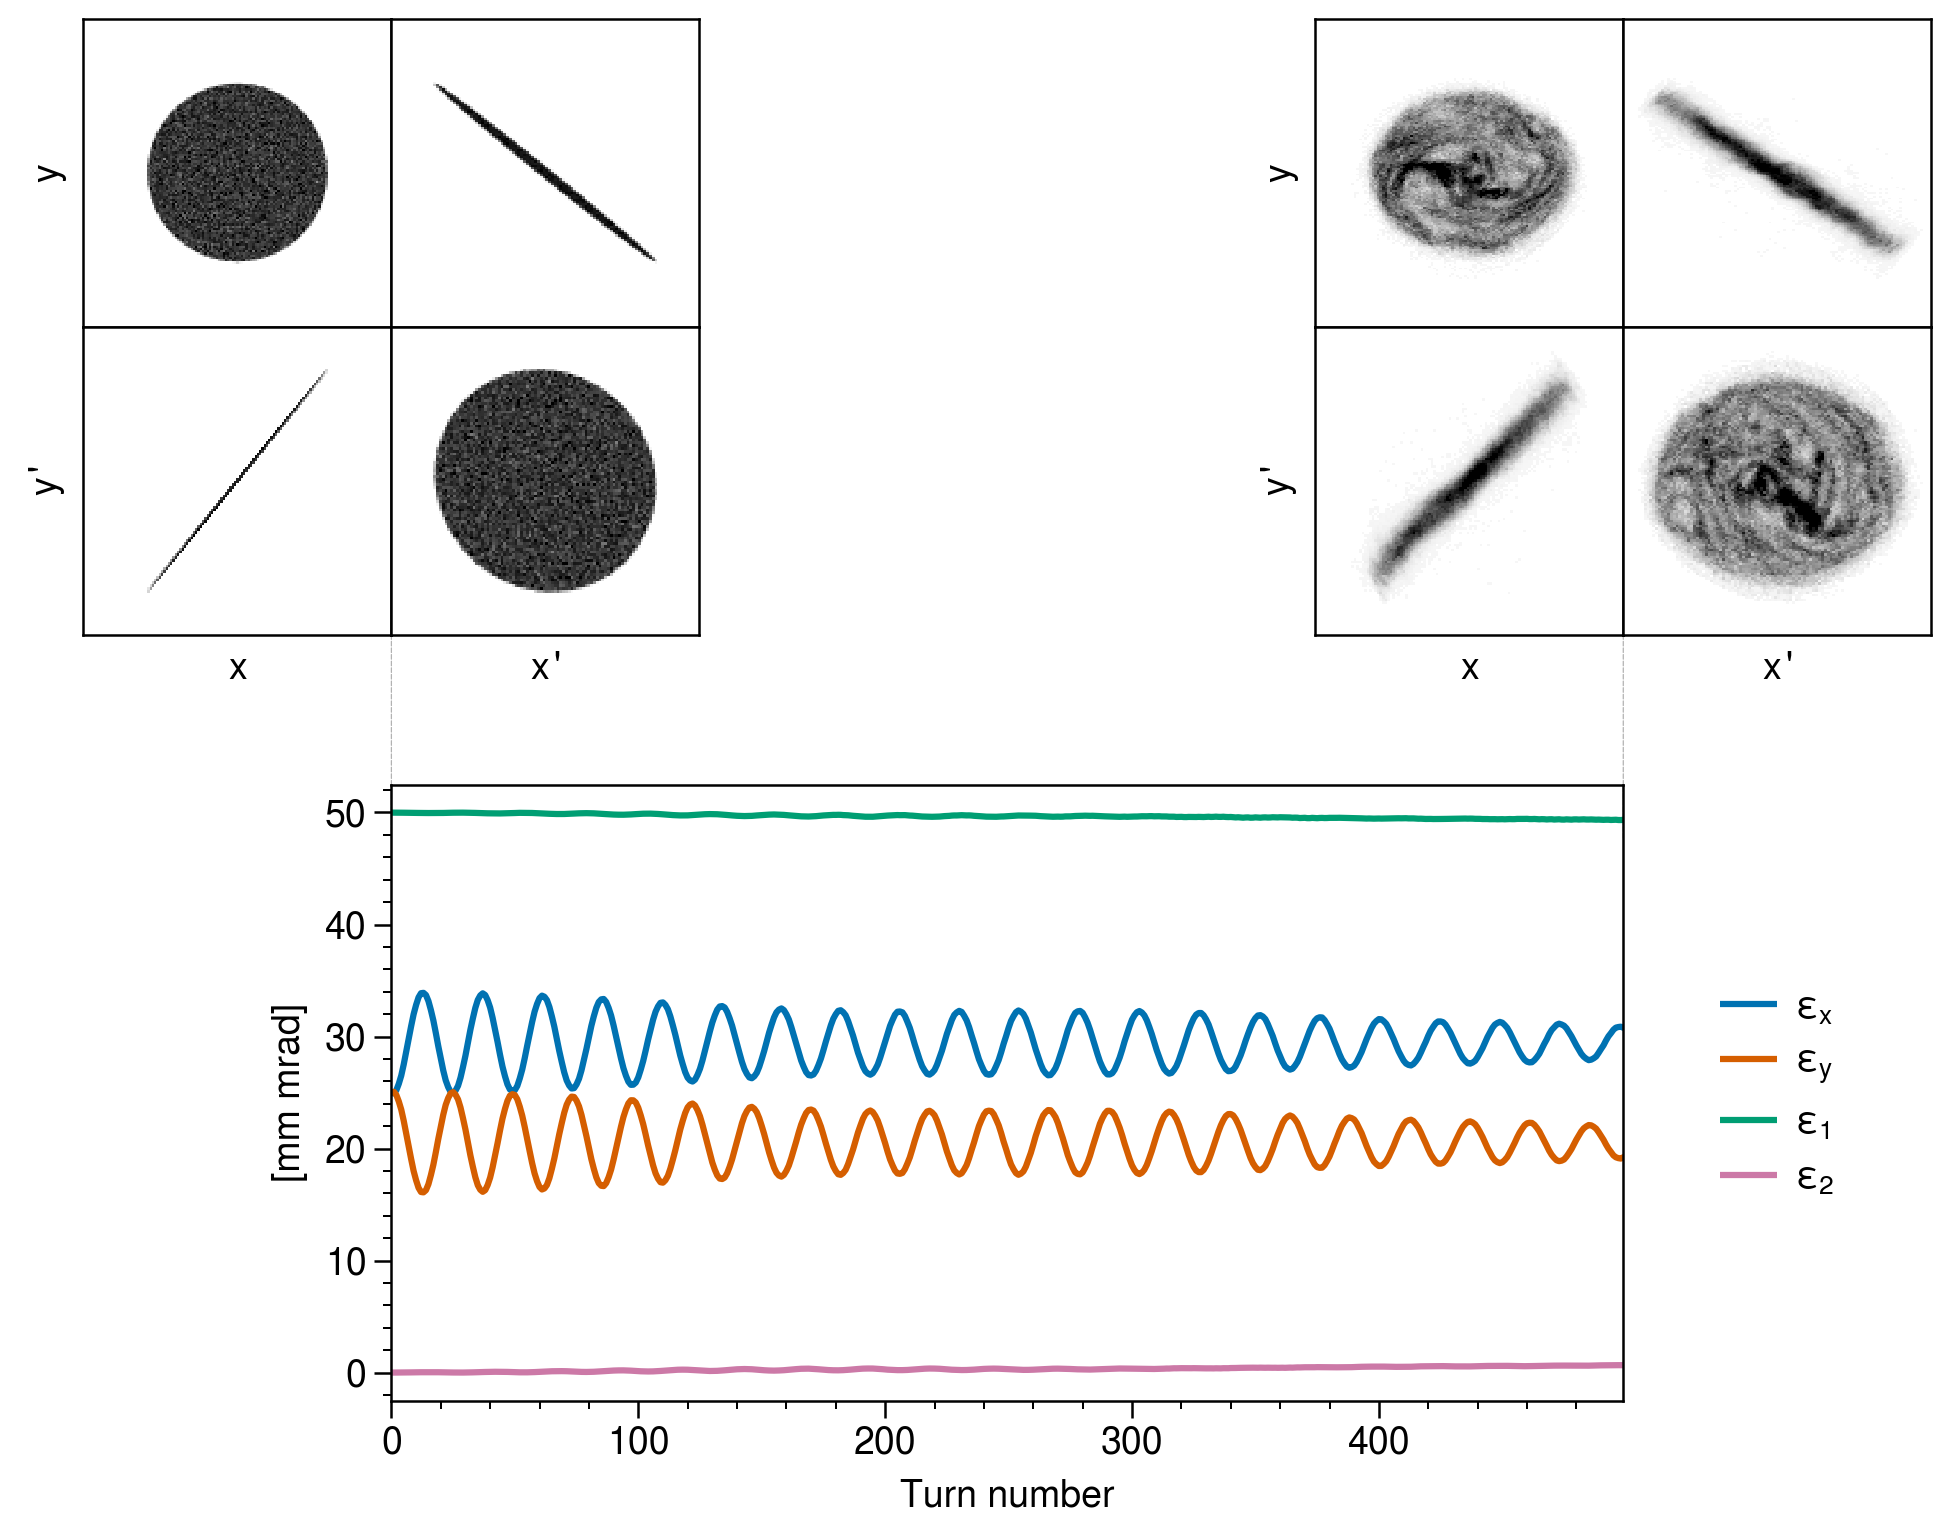
\includegraphics[width=0.7\textwidth]{Images/chapter3/fringe_spacecharge.png}
    \caption{Danilov distribution tracked in the SNS ring with space charge. Fringe fields are the only nonlinear external effect.}
    \label{fig:fringe_c}
    \vspace*{3cm}
\end{figure}